\documentclass[a4paper,11pt]{report}
\usepackage{fullpage}

\usepackage{"../../info/packages"}
\usepackage{"../../info/nomenclature"}

\usepackage{scalerel}
\usepackage{subfiles}

\newcommand{\xvecdot}{\dot{\xvec}}
\newcommand{\xdot}{\dot{x}}
\newcommand{\qvecdot}{\dot{\qvec}}
\newcommand{\qdot}{\dot{q}}

\setlength{\cellspacetoplimit}{3pt}
\setlength{\cellspacebottomlimit}{3pt}

\title{Magnetic Fields}
\author{Alejandro Campos}

\begin{document}
\maketitle
\tableofcontents

%########################################################################
\chapter{Guiding center theory}
%########################################################################
We begin with the velocity equation for a particle under the action of electric and magnetic fields, 
\begin{equation}
\label{eq:single_particle_motion}
    m \frac{d \vvec}{dt} = e \left ( \Evec + \vvec \times \Bvec \right )_{\qvec = \xvec}.
\end{equation}
In the above, $\vvec = \vvec(t)$ is the particle velocity, $\xvec = \xvec(t)$ the particle position, $\Evec = \Evec(\qvec,t)$ the electric field, and $\Bvec = \Bvec(\qvec,t)$ the magnetic field. In the subsections that follow, we will solve this equation of motion for simplified forms of $\Evec$ and $\Bvec$. The solutions for the velocity vector will typically be of the form
\begin{equation}
    \label{eq:single_particle_motion_vel_general}
    \vvec = \vvec^{(c)} + \vvec^{(g)} + v^{||} \bvec,
\end{equation}
where $\vvec^{(c)} = \vvec^{(c)}(t)$ is the gyro-motion (cyclotron) velocity, $\vvec^{(g)} = \vvec^{(g)}(t)$ is the guiding center velocity, $v^{||} = v^{||}(t)$ is the parallel velocity. Not all of the velocities will always be present. $\bvec = \Bvec / B$ is the unit magnetic field vector. The position of the particle is governed by 
\begin{equation}
    \frac{d\xvec}{dt} = \vvec.
\end{equation}
Using \cref{eq:single_particle_motion_vel_general}, we integrate the above to obtain
\begin{equation}
    \label{eq:single_particle_motion_pos_eq_mod}
    \int_0^t \, d\xvec(t') = \int_0^t \vvec^{(c)}(t') \, dt' + \int_0^t \vvec^{(g)}(t') \, dt' + \int_0^t v^{||}(t) \bvec \, dt'.
\end{equation}
We introduce the positions $\xvec^{(c)} = \xvec^{(c)}(t)$, $\xvec^{(g)} = \xvec^{(g)}(t)$, and $\xvec^{||} = \xvec^{||}(t)$, which are defined as follows
\begin{equation}
    \xvec^{(c)} = \int \vvec^{(c)} \, dt,
\end{equation}
\begin{equation}
    \xvec^{(g)} = \int \vvec^{(g)} \, dt,
\end{equation}
\begin{equation}
    \xvec^{||} = \int v^{||} \bvec \, dt.
\end{equation}
Thus, \cref{eq:single_particle_motion_pos_eq_mod} is now re-written as
\begin{equation}
    \xvec(t) - \xvec(0) = \xvec^{(c)}(t) - \xvec^{(c)}(0) + \xvec^{(g)}(t) - \xvec^{(g)}(0) - \xvec^{||}(t) - \xvec^{||}(0).
\end{equation}
Without loss of generality, we will assume that the initial condition is as follows
\begin{equation}
    \xvec(0) = \xvec^{(c)}(0) + \xvec^{(g)}(0) + \xvec^{||}(0).
\end{equation}
Thus, the particle position is finally expressed as
\begin{equation}
    \label{eq:single_particle_motion_pos_general}
    \xvec = \xvec^{(c)} + \xvec^{(g)} + \xvec^{||}.
\end{equation}

%------------------------------------------------------------------------
\section{Uniform $\Evec$ and $\Bvec$ fields}
%------------------------------------------------------------------------

%--------------------------------------------
\subsection{Only $\Evec$ field}
%--------------------------------------------
Let's orient our coordinate system such that $\Evec$ points in the $\evec_z$ direction. Thus, the equations of motion are
\begin{alignat}{2}
    &\frac{d v_x}{dt} = 0  \qquad && v_x(0) = v_\perp \cos(\phi), \nonumber \\
    &\frac{d v_y}{dt} = 0  \qquad && v_y(0) = v_\perp \sin(\phi), \nonumber \\
    &\frac{d v_z}{dt} = \frac{e E}{m}  \qquad && v_z(0) = v_{||}.
\end{alignat}
The solution of the above is
\begin{align}
    v_x &= v_\perp \cos(\phi) \nonumber \\
    v_y &= v_\perp \sin(\phi) \nonumber \\
    v_z &= v_{||} + \frac{e E}{m} t.
\end{align}

%--------------------------------------------
\subsection{Only $\Bvec$ field}
%--------------------------------------------
\begin{figure}[ht]
    \centering
    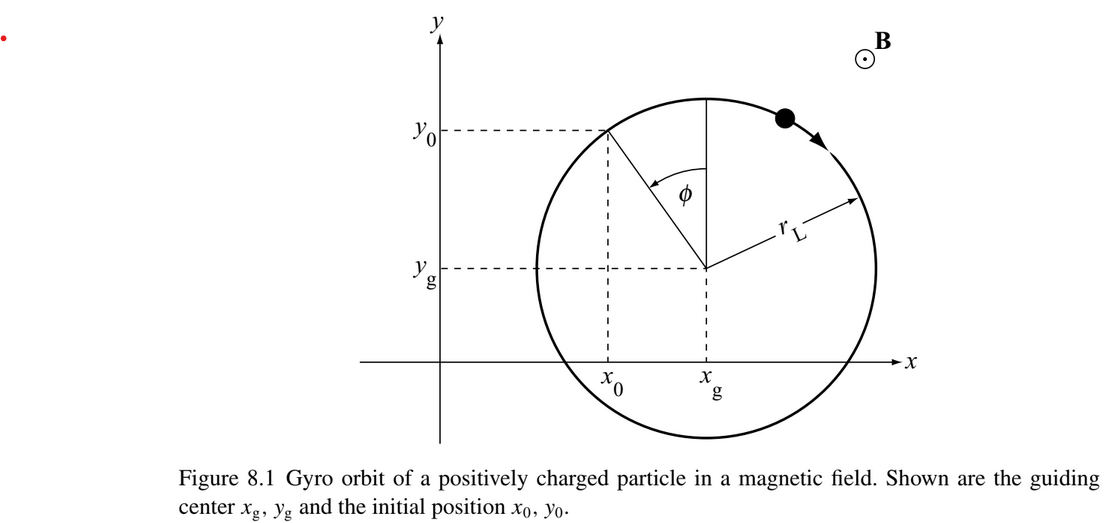
\includegraphics[width=\textwidth]{../../images/gyromotion_coordinates.png}
    \caption{Coordinates for gyro-motion (extracted from Plasma Physics and Fusion Energy, J. P. Freidberg).}
    \label{fig:gyromotion_coordiantes}
\end{figure}

\label{sec:only_B_field}
Let's orient our coordinate system such that $\Bvec$ points in the $\evec_z$ direction. Thus, the equations of motion are
\begin{subequations}
\begin{alignat}{2}
    &\frac{d v_x}{dt} = \frac{eB}{m} v_y  \qquad && v_x(0) = v_\perp \cos(\phi), \label{eq:only_B_1} \\
    &\frac{d v_y}{dt} = -\frac{eB}{m} v_x  \qquad && v_y(0) = v_\perp \sin(\phi), \label{eq:only_B_2} \\
    &\frac{d v_z}{dt} = 0  \qquad && v_z(0) = v_{||}. \label{eq:only_B_3}
\end{alignat}
\end{subequations}
The $z$ component is decoupled from the rest and has a trivial solution. For the other two components, we begin by taking the time derivative of \cref{eq:only_B_2}. Thus
\begin{equation}
    \frac{d^2 v_y}{dt^2} = -\frac{eB}{m} \frac{d v_x}{dt} = -w_c^2 v_y,
\end{equation}
where $w_c = |e|B/m$ is the gyro frequency. We know that the general solution to the above is $v_y = c_1 \cos(w_c t) + c_2 \sin(w_c t)$. If we use the ICs and assume ions, we have
\begin{equation}
\label{eq:vel_gyro_y}
    v_y = -v_\perp \sin(w_ct - \phi).
\end{equation}
Integrating \cref{eq:only_B_1} then gives
\begin{equation}
\label{eq:vel_gyro_x}
    v_x = v_\perp \cos(w_c t - \phi).
\end{equation}
The final solution, for either positive or negative charges, can be written as
\begin{align}
\label{eq:vel_gyro}
    v^{(c)}_x &= v_\perp \cos(w_c t \pm \phi) \nonumber \\
    v^{(c)}_y &= \pm v_\perp \sin(w_c t \pm \phi),
\end{align}
where upper signs correspond to a negative charge. Integrating the equations above leads to
\begin{align}
\label{eq:pos_gyro}
    x^{(c)} &= r_L \sin(w_c t \pm \phi) \nonumber \\
    y^{(c)} &= \mp r_L \cos(w_c t \pm \phi).
\end{align}
where $r_L = v_\perp/w_c$ is the gyro radius.

%--------------------------------------------
\subsection{Both $\Evec$ and $\Bvec$ fields}
%--------------------------------------------
\label{sec:E_and_B_field}
Let's orient our coordinate system such that $\Bvec$ still points along $\evec_z$. The equations of motion are
\begin{subequations}
\label{eq:single_particle_motion_EcrossB_temp1}
\begin{alignat}{2}
    &\frac{d v_x}{dt} = \frac{eE_x}{m} + \frac{eB}{m} v_y  \qquad && v_x(0) = v_\perp \cos(\phi) + \frac{E_y}{B}, \label{eq:E_and_B_1} \\
    &\frac{d v_y}{dt} = \frac{eE_y}{m} - \frac{eB}{m} v_x  \qquad && v_y(0) = v_\perp \sin(\phi) - \frac{E_x}{B}, \label{eq:E_and_B_2} \\
    &\frac{d v_z}{dt} = \frac{e E_{||}}{m}  \qquad && v_z(0) = v_{||}, \label{eq:E_and_B_3}
\end{alignat}
\end{subequations}
where we have chosen the given initial conditions simply to facilitate the math. Again, the z component is decoupled from the rest and has the trivial solution $v_z = v_{||} +  (eE_{||}/m) t$. Thus, \cref{eq:single_particle_motion_vel_general} for the $x$ and $y$ components are
\begin{align}
    \label{eq:single_particle_motion_EcrossB_temp2}
    v_x &= v_x^{(c)} + v^{(g)}_x, \nonumber \\
    v_y &= v_y^{(c)} + v^{(g)}_y.
\end{align}
We assume $v^{(g)}_x$ and $v^{(g)}_y$ are time independent. Using \cref{eq:single_particle_motion_EcrossB_temp2} in \cref{eq:single_particle_motion_EcrossB_temp1} we obtain
\begin{align}
    0 &= \frac{eE_x}{m} + \frac{eB}{m}v^{(g)}_y \nonumber \\
    0 &= \frac{eE_y}{m} - \frac{eB}{m}v^{(g)}_x.
\end{align}
Thus, $v^{(g)}_x = E_y/B$ and $v^{(g)}_y = -E_x/B$, which in vector notation can be expressed as
\begin{equation}
    \vvec^{(g)}_E = \frac{\Evec \times \Bvec}{B^2}.
\end{equation}

%------------------------------------------------------------------------
\section{Non-uniform $\Bvec$ field}
%------------------------------------------------------------------------

%--------------------------------------------
\subsection{Change in magnitude along perpendicular directions}
%--------------------------------------------
The magnetic field still points in the $\evec_z$ direction, but its magnitude changes in directions perpendicular to $\evec_z$: $B = B(q_x,q_y)$. The equations of motion are
\begin{subequations}
\begin{alignat}{2}
    &\frac{d v_x}{dt} = \frac{eB(x,y)}{m} v_y  \qquad && v_x(0) = v_\perp \cos(\phi) -\frac{v^2_\perp}{2 w_c} \left . \frac{\partial B}{\partial q_y} \right |_{x^{(g)},y^{(g)}} \frac{1}{B(x^{(g)},y^{(g)})}, \label{eq:nonuniB_1} \\
    &\frac{d v_y}{dt} = -\frac{eB(x,y)}{m} v_x  \qquad && v_y(0) = v_\perp \sin(\phi) + \frac{v^2_\perp}{2 w_c} \left . \frac{\partial B}{\partial q_x} \right |_{x^{(g)},y^{(g)}} \frac{1}{B(x^{(g)},y^{(g)})}, \label{eq:nonuniB_2} \\
    &\frac{d v_z}{dt} = 0  \qquad && v_z(0) = v_{||}. \label{eq:nonuniB_3}
\end{alignat}
\end{subequations}
In the above, the $x$ and $y$ in $B(x,y)$ are the perpendicular components of the particle's position. The $v_z$ component is decoupled from the rest and has a trivial solution. Thus, \cref{eq:single_particle_motion_vel_general,eq:single_particle_motion_pos_general} for the $x$ and $y$ components are
\begin{equation}
    \label{eq:single_particle_motion_vel_Bmag_change_perp_1}
    v_x = v_x^{(c)} + v_x^{(g)},
\end{equation}
\begin{equation}
    \label{eq:single_particle_motion_vel_Bmag_change_perp_2}
    v_y = v_y^{(c)} + v_y^{(g)},
\end{equation}
\begin{equation}
    \label{eq:single_particle_motion_pos_Bmag_change_perp_1}
    x = x^{(c)} + x^{(g)},
\end{equation}
\begin{equation}
    \label{eq:single_particle_motion_pos_Bmag_change_perp_2}
    y = y^{(c)} + y^{(g)}.
\end{equation}

We begin by employing a Taylor-series expansion for the magnetic field
\begin{equation}
    B(x,y) = B(x^{(g)}, y^{(g)}) + \left . \frac{\partial B}{\partial q_x} \right |_{x^{(g)},y^{(g)}} x^{(c)} + \left . \frac{\partial B}{\partial q_y} \right |_{x^{(g)},y^{(g)}} y^{(c)} + ...
\end{equation}
Thus, \cref{eq:nonuniB_1,eq:nonuniB_2} are now
\begin{equation}
    \frac{ d v_x}{dt} = \frac{e B(x^{(g)},y^{(g)})}{m} v_y + \frac{e}{m} \left ( \left . \frac{\partial B}{\partial q_x} \right|_{x^{(g)},y^{(g)}} x^{(c)} + \left . \frac{\partial B}{\partial q_y} \right |_{x^{(g)},y^{(g)}} y^{(c)} \right) v_y
\end{equation}
\begin{equation}
    \frac{ d v_y}{dt} = -\frac{e B(x^{(g)},y^{(g)})}{m} v_x + \frac{e}{m} \left ( \left . \frac{\partial B}{\partial q_x} \right|_{x^{(g)},y^{(g)}} x^{(c)} + \left . \frac{\partial B}{\partial q_y} \right |_{x^{(g)},y^{(g)}} y^{(c)} \right ) v_x.
\end{equation}
As before, we assume $v_x^{(g)}$, $v_y^{(g)}$ are time independent. Also, for simplicity we assume ions only. Plugging in \cref{eq:single_particle_motion_vel_Bmag_change_perp_1,eq:single_particle_motion_vel_Bmag_change_perp_2} into the above, we get
\begin{equation}
    0 = B(x^{(g)},y^{(g)}) v_y^{(g)} + \left ( \left . \frac{\partial B}{\partial q_x} \right|_{x^{(g)},y^{(g)}} x^{(c)} + \left . \frac{\partial B}{\partial q_y} \right |_{x^{(g)},y^{(g)}} y^{(c)} \right) \left ( v_y^{(c)} + v_y^{(g)} \right),
\end{equation}
\begin{equation}
    0 = -B(x^{(g)},y^{(g)}) v_x^{(g)} + \left ( \left . \frac{\partial B}{\partial q_x} \right|_{x^{(g)},y^{(g)}} x^{(c)} + \left . \frac{\partial B}{\partial q_y} \right |_{x^{(g)},y^{(g)}} y^{(c)} \right ) \left ( v_x^{(c)} + v_x^{(g)} \right ).
\end{equation}
We assume $v_x^{(g)} \ll v_x^{(c)}$ and $v_y^{(g)} \ll v_y^{(c)}$. Thus, the above becomes
\begin{equation}
    \label{eq:single_particle_motion_Bmag_change_perp_temp1}
    0 = B(x^{(g)},y^{(g)}) v_y^{(g)} + \left ( \left . \frac{\partial B}{\partial q_x} \right|_{x^{(g)},y^{(g)}} x^{(c)} + \left . \frac{\partial B}{\partial q_y} \right |_{x^{(g)},y^{(g)}} y^{(c)} \right) v_y^{(c)},
\end{equation}
\begin{equation}
    \label{eq:single_particle_motion_Bmag_change_perp_temp2}
    0 = -B(x^{(g)},y^{(g)}) v_x^{(g)} + \left ( \left . \frac{\partial B}{\partial q_x} \right|_{x^{(g)},y^{(g)}} x^{(c)} + \left . \frac{\partial B}{\partial q_y} \right |_{x^{(g)},y^{(g)}} y^{(c)} \right ) v_x^{(c)}.
\end{equation}
We now use the definitions in \cref{eq:vel_gyro} and \cref{eq:pos_gyro}. For example, with those definitions we can show that 
\begin{align}
     x^{(c)} v_y^{(c)} &= \left[ r_L \sin (w_c t - \phi) \right] \left[ -v_\perp \sin (w_ct - \phi) \right] \nonumber \\
    & = -\frac{ v^2_\perp}{w_c} \sin^2(w_c t - \phi) \nonumber \\
    & = -\frac{ v^2_\perp}{2 w_c} \{1 - \cos [ 2 (w_c t - \phi)] \}
\end{align}
Similar derivations can be carried out for $y^{(c)} v_y^{(c)}$, $x^{(c)} v_x^{(c)}$, and $y^{(c)} v_x^{(c)}$. Thus, \cref{eq:single_particle_motion_Bmag_change_perp_temp1,eq:single_particle_motion_Bmag_change_perp_temp2} become 
\begin{multline}
    0 = B(x^{(g)},y^{(g)}) v_y^{(g)} -\frac{ v^2_\perp}{2 w_c} \left . \frac{\partial B}{\partial q_x} \right |_{x^{(g)},y^{(g)}} \{1 - \cos [ 2 (w_c t - \phi)] \} \\
    - \frac{ v^2_\perp}{2 w_c} \left .\frac{\partial B}{\partial q_y} \right |_{x^{(g)},y^{(g)}} \sin [ 2(w_ct - \phi)],
\end{multline}
\begin{multline}
    0 = -B(x^{(g)},y^{(g)}) v_x^{(g)} -\frac{ v^2_\perp}{2 w_c} \left . \frac{\partial B}{\partial q_x} \right |_{x^{(g)},y^{(g)}} \sin [ 2 (w_c t - \phi)] \\
    - \frac{ v^2_\perp}{2 w_c} \left .\frac{\partial B}{\partial q_y} \right |_{x^{(g)},y^{(g)}} \{ 1 + \cos [ 2(w_ct - \phi)] \}.
\end{multline}
We neglect the oscillatory terms containing the sines and cosines---if it was not possible to neglect them, then the assumption that $v^{(g)}_x$, $v^{(g)}_y$ are time independent would not hold. Thus,
\begin{subequations}
\begin{alignat}{2}
    0 &= B(x^{(g)},y^{(g)}) v_y^{(g)} - \frac{ v^2_\perp}{2 w_c} \left . \frac{\partial B}{\partial q_x} \right |_{x^{(g)},y^{(g)}} \nonumber \\
    0 &= -B(x^{(g)},y^{(g)}) v_x^{(g)} -\frac{ v^2_\perp}{2 w_c} \left . \frac{\partial B}{\partial q_y} \right |_{x^{(g)},y^{(g)}} . 
\end{alignat}
\end{subequations}
Solving for the guiding center velocities, we finally have
\begin{align}
    v_x^{(g)} &= -\frac{v^2_\perp}{2 w_c} \left . \frac{\partial B}{\partial q_y} \right |_{x^{(g)},y^{(g)}} \frac{1}{B(x^{(g)},y^{(g)})} \nonumber \\
    v_y^{(g)} &= \frac{v^2_\perp}{2 w_c} \left . \frac{\partial B}{\partial q_x} \right |_{x^{(g)},y^{(g)}} \frac{1}{B(x^{(g)},y^{(g)})} . 
\end{align}
In vector notation, this is written as
\begin{equation}
    \vvec^{(g)}_{\nabla B} = \mp \frac{v^2_\perp}{2 w_c} \frac{ \Bvec \times \nabla B }{B^2}.
\end{equation}
In the above, the fields and $w_c$ are evaluated at $(x^{(g)},y^{(g)})$.

%--------------------------------------------
\subsection{Change in magnitude along parallel directions}
%--------------------------------------------
Ideally, one would introduce a gradient only in the direction parallel to the magnetic field, that is, one would have $\Bvec = B(q_z) \evec_z$. However, due to Gauss's law, this is too restrictive and instead we generalize and use $\Bvec = B_x \evec_x + B_z \evec_z$, where $B_x = B_x(q_x,q_z)$ and $B_z = B_z(q_x,q_z)$. Thus, the equations of motion are
\begin{align}
    \frac{dv_x}{dt} &= \frac{e}{m} v_y B_z(x,z) , \label{eq:par_grad_vx_inter}\\
    \frac{dv_y}{dt} &= -\frac{e}{m} [v_x B_z(x,z) - v_z B_x(x,z)] , \label{eq:par_grad_vy_inter}\\
    \frac{dv_z}{dt} &= -\frac{e}{m} v_y B_x(x,z) \label{eq:par_grad_vz_inter}.
\end{align}
However, the $z$ direction no longer corresponds to the parallel direction, since the magnetic field also has a component along the $x$ direction. To account for this, we will introduce a rotating reference frame, in which one of the axis will always be aligned with the magnetic field vector, and thus would denote the parallel direction. In the original static reference frame the unit vectors are $(\evec_x, \evec_y, \evec_z)$ and the velocity components are $(v_x, v_y, v_x)$, whereas in this new rotating reference frame the unit vectors are $(\evec_{\perp1}, \evec_{\perp2}, \bvec)$ and the velocity components are $(v_{\perp1}, v_{\perp2}, v_{||})$. 

The rotating reference frame is described by the rotation matrix
\begin{equation}
    \Qvec(t) = \begin{bmatrix} b_x & 0 & b_z \\ 0 & 1 & 0 \\ b_z & 0 & -b_x \end{bmatrix},
\end{equation}
where $b_x = b_x(t)$ and $b_y = b_y(t)$ are given by
\begin{equation}
    b_x = \frac{B_x(x,z)}{B(x,z)} \qquad b_z = \frac{B_z(x,z)}{B(x,z)} \label{eq:bvec_components}
\end{equation}
In the above, $B(x,z) = [ B_x^2(x,z) + B_z^2(x,z) ]^{1/2}$. As an example, the matrix above leads to the following transformations for the unit vectors and velocities in the rotating reference frame 
\begin{align}
    \bvec &= b_x \evec_x + b_z \evec_z \\
    \evec_{\perp2} &= \evec_y \\
    \evec_{\perp1} &= b_z \evec_x - b_x \evec_z = \evec_{\perp2} \times \bvec,
\end{align}
\begin{align}
    v_{||} &= b_x v_x + b_z v_z \label{eq:par_grad_vel_trans_1}\\
    v_{\perp2} &= v_y \label{eq:par_grad_vel_trans_2}\\
    v_{\perp1} &= b_z v_x - b_x v_z. \label{eq:par_grad_vel_trans_3}
\end{align}
Using the transformation rule for the acceleration of a particle, but for some reason neglecting the coriollis and centrifugal forces, we obtain for the velocity derivatives
\begin{align}
    \frac{dv_{||}}{dt} &= \frac{dv_x}{dt} b_x + \frac{dv_z}{dt} b_z  - K v_{\perp1} \\
    \frac{dv_{\perp2}}{dt} &= \frac{dv_y}{dt}\\
    \frac{dv_{\perp1}}{dt} &= \frac{dv_x}{dt} b_z - \frac{dv_z}{dt} b_x + K v_{||},
\end{align}
where $K = K(t)$ is given by $K = b_x db_z/dt - b_z db_x/dt$. Using \cref{eq:par_grad_vx_inter,eq:par_grad_vy_inter,eq:par_grad_vz_inter} in the above leads to
\begin{align}
    \frac{d v_{||}}{dt} &= \frac{e}{m} v_y [B_z(x,z) b_x - B_x(x,z) b_z] - Kv_{\perp1} \\
    \frac{dv_{\perp2}}{dt} &= -\frac{eB}{m} (v_x b_z - v_z b_x) \\
    \frac{dv_{\perp1}}{dt} &= \frac{e}{m} v_y [B_z(x,z) b_z + B_x(x,z) b_x] + Kv_{||} 
\end{align}
Using the definitions for $b_x$ and $b_z$ in \cref{eq:bvec_components}, as well as the expressions for $v_{\perp1}$, $v_{\perp2}$ in \cref{eq:par_grad_vel_trans_2,eq:par_grad_vel_trans_3}, we get
\begin{align}
    \frac{d v_{||}}{dt} &= -Kv_{\perp1}, \label{eq:par_grad_vpar_inter} \\
    \frac{dv_{\perp2}}{dt} &= -w_c v_{\perp1}, \label{eq:par_grad_v2_inter} \\
    \frac{dv_{\perp1}}{dt} &= w_c v_{\perp2} + K v_{||}, \label{eq:par_grad_v1_inter}
\end{align}
where $w_c = w_c(t)$ is given by $w_c = e B(x,z) / m$.

We now introduce a time transformation to simplify the equations above. To do so, we introduce the following variables
\begin{gather}
    \hat{v}_{||} = \hat{v}_{||}(\tau) \qquad \hat{v}_{\perp2} = \hat{v}_{\perp2}(\tau) \qquad \hat{v}_{\perp1} = \hat{v}_{\perp1}(\tau) \\
    \hat{x} = \hat{x}(\tau) \qquad \hat{z} = \hat{z}(\tau)
\end{gather}
such that
\begin{gather}
    v_{||} = \hat{v}_{||}(h(t)) \qquad v_{\perp2} = \hat{v}_{\perp2}(h(t)) \qquad v_{\perp1} = \hat{v}_{\perp1}(h(t)) \\
    x = \hat{x}(h(t)) \qquad z = \hat{z}(h(t)).
\end{gather}
The function $h(t)$ is given by
\begin{equation}
    h(t) = \int_0^t w_c(t') dt'.
\end{equation}
We also show that
\begin{equation}
    b_x = \frac{B_x(x,z)}{B(x,z)} = \frac{B_x(\hat{x}(h(t)),\hat{z}(h(t)))}{B(\hat{x}(h(t)),\hat{z}(h(t)))},
\end{equation}
and thus
\begin{equation}
    \frac{db_x}{dt} = \frac{dh(t)}{dt} \frac{d}{d\tau} \left [ \frac{B_x(\hat{x},\hat{z})}{B(\hat{x},\hat{z})} \right ]_{\tau = h(t)} = w_c \left .\frac{d \hat{b}_x}{d\tau} \right|_{\tau = h(t)},
\end{equation}
where $\hat{b}_x =\hat{b}_x(\tau)$ is given by $\hat{b}_x= B_x(\hat{x},\hat{z}) / B(\hat{x},\hat{z})$. The analogous holds for $b_z$. This allows us to write
\begin{equation}
    K = w_c \left ( \hat{b}_x \frac{d\hat{b}_z}{d \tau} - \hat{b}_z \frac{d\hat{b}_x}{d \tau} \right )_{\tau = h(t)} = w_c \left. \hat{K} \right |_{\tau = h(t)},
\end{equation}
where $\hat{K} = \hat{K}(\tau)$ is given by $\hat{K} = \hat{b}_x d\hat{b}_z/d\tau - \hat{b}_z d\hat{b}_x/d\tau$. With these transformation, \cref{eq:par_grad_vpar_inter,eq:par_grad_v2_inter,eq:par_grad_v1_inter} are re-written as
\begin{align}
    \frac{d\hat{v}_{||}}{d\tau} &= -\hat{K} \hat{v}_{\perp1},\\
    \frac{d\hat{v}_{\perp2}}{d\tau} &= -\hat{v}_{\perp1},\\
    \frac{d\hat{v}_{\perp1}}{d\tau} &= \hat{v}_{\perp2} + \hat{K} \hat{v}_{||}.
\end{align}

We now simplify $B_z$ so that $B_z = B_z(q_z)$. To be consistent with Gauss's law, we require $B_x = B_x(q_x,q_y)$ where $B_x = -q_x dB_z/dq_z$. With these simplified forms, we have
\begin{align}
    \hat{K} &= -\hat{b}_z^2 \frac{d}{d\tau} \left ( \frac{\hat{b}_x}{\hat{b}_z} \right ) \\
    &= -\frac{B_z^2(\hat{z})}{B^2(\hat{x},\hat{z})} \frac{d}{d\tau} \left ( \frac{B_x(\hat{x},\hat{z})}{B_z(\hat{z})} \right ) \\
    &= \frac{B_z^2(\hat{z})}{B^2(\hat{x},\hat{z})} \frac{d}{d\tau} \left [ \hat{x}  \left ( \frac{1}{B_z} \frac{dB_z}{dq_z} \right )_{q_z = \hat{z}} \right ].
\end{align}
We now use the long-thin approximation. For this approximation, we assume that $B_x / B_z \ll 1$, and also that $\frac{1}{B_z} \frac{dB_z}{dq_z}$ changes very slowly. We thus have
\begin{equation}
\label{eq:par_grad_k_inter}
    \hat{K} \approx \frac{d \hat{x}}{d\tau} \left ( \frac{1}{B_z} \frac{dB_z}{dq_z} \right)_{q_z = \hat{z}}.
\end{equation}
Also, using the long-thin approximation in \cref{eq:par_grad_vel_trans_1,eq:par_grad_vel_trans_3} allows us to write
\begin{align}
    v_{||} &\approx v_z = \frac{dz}{dt} = \left ( \frac{d\hat{z}}{d\tau} \right )_{\tau = h(t)} w_c \\
    v_{\perp1} & \approx v_x = \frac{dx}{dt} = \left ( \frac{d \hat{x}}{d\tau} \right )_{\tau = h(t)} w_c.
\end{align}
Evaluating the above at $t = h^{-1}(\tau)$, and defining $\hat{w}_c(\tau)$ from $w_c = \hat{w}_c(h(t))$, we obtain
\begin{align}
    \hat{v}_{||} &\approx  \frac{d\hat{z}}{d\tau}  \hat{w}_c \\
    \hat{v}_{\perp1} & \approx \frac{d \hat{x}}{d\tau} \hat{w}_c.
\end{align}
We also note that
\begin{equation}
    \frac{d B_z(\hat{z})}{d\tau} = \left ( \frac{dB_z}{dq_z} \right )_{q_z = \hat{z}} \frac{d \hat{z}}{d\tau}.
\end{equation}
Using the expressions above in \cref{eq:par_grad_k_inter}, one can approximate $\hat{K}$ using either of the two forms below
\begin{equation}
    \hat{K} \approx \frac{\hat{v}_{\perp1}}{\hat{w}_c B_z(\hat{z})} \left ( \frac{dB_z}{dq_z} \right )_{q_z = \hat{z}} \approx \frac{\hat{v}_{\perp1}}{\hat{v}_{||} B_z(\hat{z})} \frac{dB_z(\hat{z})}{d\tau} .
\end{equation}
We thus write the governing equations for the velocities as
\begin{align}
    \frac{d\hat{v}_{||}}{d\tau} &= -\frac{\hat{v}^2_{\perp1}}{\hat{w}_c B_z(\hat{z})} \left ( \frac{dB_z}{dq_z} \right )_{q_z = \hat{z}} ,\label{eq:par_grad_vpar_thin}\\
    \frac{d\hat{v}_{\perp2}}{d\tau} &= -\hat{v}_{\perp1}, \label{eq:par_grad_v2_thin} \\
    \frac{d\hat{v}_{\perp1}}{d\tau} &= \hat{v}_{\perp2} + \frac{\hat{v}_{\perp1}}{B_z(\hat{z})} \frac{dB_z(\hat{z})}{d\tau}. \label{eq:par_grad_v1_thin}
\end{align}

We now assume the solution for the perpendicular velocities is of the form
\begin{align}
    \hat{v}_{\perp1} &= \hat{v}_\perp \cos [\tau + \hat{\epsilon}] \\
    \hat{v}_{\perp2} &= -\hat{v}_\perp \sin [\tau + \hat{\epsilon}],
\end{align}
where $\hat{v}_\perp = \hat{v}_\perp(\tau)$ and $\hat{\epsilon} = \hat{\epsilon}(\tau)$. Plugging these two assumed solutions into \cref{eq:par_grad_v2_thin,eq:par_grad_v1_thin}, and using some simple algebra, gives
\begin{equation}
    \frac{d\hat{v}_\perp}{d\tau} = \frac{\hat{v}_\perp}{2 B_z(\hat{z})} \frac{dB_z(\hat{z})}{d\tau} \left \{ 1 + \cos [2 (\tau + \hat{\epsilon})] \right \}.
\end{equation}
The above can be re-arranged and expressed as
\begin{equation}
\label{eq:par_grad_mu_evol}
    \frac{d \ln \hat{\mu}}{d\tau} = \frac{d \ln B_z(\hat{z}) }{d\tau} \cos [2 (\tau + \hat{\epsilon})],
\end{equation}
where $\hat{\mu} = \hat{\mu}(\tau)$ is the adiabatic invariant, and is given by
\begin{equation}
    \hat{\mu} = \frac{m \hat{v}^2_\perp}{2 B_z(\hat{z})}.
\end{equation}
Integrating \cref{eq:par_grad_mu_evol} from $\tau_1$ to $\tau_2$ gives
\begin{equation}
    \ln \hat{\mu}(\tau_2) - \ln \hat{\mu}(\tau_1) = \left . \ln [B_z(\hat{z})] \cos [2(\tau + \hat{\epsilon})] \right |^{\tau_2}_{\tau_1} + \int_{\tau_1}^{\tau_2} 2 \ln [ B_z(\hat{z}) ] \sin [2(\tau + \hat{\epsilon})] d\tau.
\end{equation}
Picking $\tau_1$ and $\tau_2$ such that $[\tau_2 + \hat{\epsilon}(\tau_2)] - [\tau_1 + \hat{\epsilon}(\tau_1)] = 2 \pi$, and assuming $B(\hat{z})$ doesn't change significantly from $\tau_1$ to $\tau_2$, gives $\hat{\mu}(\tau_2) = \hat{\mu}(\tau_1)$, that is, $\hat{\mu}$ is constant over one gyro-period. One can also define
\begin{equation}
    \mu = \frac{m v_\perp^2}{2B_z(z)}
\end{equation}
where $\mu = \mu(t)$ and $v_\perp = v_\perp(t)$. Given that $v_\perp = \hat{v}_\perp(h(t))$, we have $\mu = \hat{\mu}(h(t))$. Thus, $\hat{\mu}(\tau_2) = \hat{\mu}(\tau_1)$ translates to $\mu(t_2) = \mu(t_1)$, where $t_2 = h^{-1}(\tau_2)$ and $t_1 = h^{-1}(\tau_1)$.

Finally, we focus not on the perpendicular velocities but the parallel velocity. Plugging-in the assumed solutions in the governing \cref{eq:par_grad_vpar_thin} gives
\begin{equation}
    \frac{d\hat{v}_{||}}{d\tau} = -\frac{\hat{v}^2_{\perp}}{2\hat{w}_c B_z(\hat{z})} \left ( \frac{dB_z}{dq_z} \right )_{q_z = \hat{z}} \{ 1 + \cos [2(\tau + \hat{\epsilon})] \}.
\end{equation}
We now average the above from $\tau_1$ to $\tau_2$ while assuming $B(\hat{z})$, $d\hat{v}_{||}/d\tau$ and $\hat{v}^2_\perp$ do not change significantly during that time scale. Note that since this is an average, we are not just integrating from $\tau_1$ to $\tau_2$, but we are also dividing by $\tau_2 - \tau_1$. After  averaging, we obtain
\begin{equation}
    \frac{d\hat{v}_{||}}{d\tau} = -\frac{\hat{v}^2_{\perp}}{2\hat{w}_c B_z(\hat{z})} \left ( \frac{dB_z}{dq_z} \right )_{q_z = \hat{z}} .
\end{equation}
or
\begin{equation}
    m \frac{d\hat{v}_{||}}{d\tau} = -\frac{\hat{\mu}}{\hat{w}_c} \left ( \frac{dB_z}{dq_z} \right )_{q_z = \hat{z}} .
\end{equation}
Converting back to time $t$ gives
\begin{equation}
    m \frac{dv_{||}}{dt} = -\mu \left ( \frac{dB_z}{dq_z} \right )_{q_z = z} .
\end{equation}


%--------------------------------------------
\subsection{Change in direction}
%--------------------------------------------
Rather than writing \cref{eq:single_particle_motion} in terns if its components as done in previous sections, we leave the equation in vector form. Expressing the velocity as $\vvec = \vvec_\perp + v_{||} \bvec$ and assuming no electric field, we write \cref{eq:single_particle_motion} as
\begin{equation}
    \frac{d}{dt} ( \vvec_\perp + v_{||} \bvec) = \mp w_c (\vvec_\perp + v_{||} \bvec ) \times \bvec,
\end{equation}
where upper sign corresponds to negative charge and lower sign to positive charge. For simplicity we will assume positively charged particles only. We then cross both sides of the above by $\bvec$, that is
\begin{equation}
    \bvec \times \left \{ \left [ \frac{d}{dt} ( \vvec_\perp + v_{||} \bvec) - w_c ( \vvec_\perp + v_{||} \bvec) \times \bvec \right ] \times \bvec \right \} = 0.
\end{equation}
The above is simplified using the following three manipulations
\begin{align}
    \bvec \times \left \{ \left [ w_c ( \vvec_\perp + v_{||} \bvec) \times \bvec \right ] \times \bvec \right \} &= \bvec \times \left \{ \left [ w_c \vvec_\perp \times \bvec \right ] \times \bvec \right \} \nonumber \\
    & = -\bvec \times \left \{ w_c \vvec_\perp ( \bvec \cdot \bvec) - \bvec (\bvec \cdot w_c \vvec_\perp ) \right \} \nonumber \\
    & = w_c \vvec_\perp \times \bvec.
\end{align}
\begin{equation}
    \bvec \times \left \{ \left [ \frac{d\vvec_\perp}{dt} \right ] \times \bvec \right \} = \frac{d \vvec_\perp}{dt}( \bvec \cdot \bvec) - \bvec \left ( \bvec \cdot \frac{d\vvec_\perp}{dt} \right ) = \left ( \frac{d \vvec_\perp}{dt} \right )_\perp.
\end{equation}
\begin{align}
    \bvec \times \left \{ \left [ \frac{d v_{||} \bvec}{dt} \times \bvec \right ] \right \} &= v_{||} \bvec \times \left \{ \left [ \frac{ d\bvec}{dt} \times \bvec \right ] \right \} \nonumber \\
    & = v_{||} \left [ \frac{d \bvec}{dt} ( \bvec \cdot \bvec) - \bvec \left ( \bvec \cdot \frac{d \bvec}{dt} \right ) \right ] \nonumber \\
    & = v_{||} \left [ \frac{d \bvec}{dt} - \bvec \left ( \frac{1}{2} \frac{d \bvec \cdot \bvec}{dt} \right ) \right ] \nonumber \\
    & = v_{||} \frac{d \bvec}{dt}
\end{align}
Thus, we have
\begin{equation}
\label{eq:curvature_1}
    \left ( \frac{ d \vvec_\perp}{dt} \right )_\perp - w_c \vvec_\perp \times \bvec = -v_{||} \frac{d\bvec}{dt}.
\end{equation}
As shown in Freidberg
\begin{equation}
    \frac{d \bvec(\xvec(t))}{dt} = \frac{d \xvec(t)}{dt} \cdot \nabla \bvec = \vvec \cdot \nabla \bvec = \vvec_\perp \cdot \nabla \bvec + v_{||} \bvec \cdot \nabla \bvec,
\end{equation}
where $\nabla \bvec$ is evaluated at $\xvec = \xvec(t)$. Thus, \cref{eq:curvature_1} becomes
\begin{equation}
\label{eq:curvature_2}
    \left ( \frac{ d \vvec_\perp}{dt} \right )_\perp - w_c \vvec_\perp \times \bvec = -v_{||} \vvec_\perp \cdot \nabla \bvec - v_{||}^2 \bvec \cdot \nabla \bvec.
\end{equation}
As was done for the other drifts, we assume the solution is of the form $\vvec_\perp = \vvec^{(c)} + \vvec^{(g)}$, where we assume again that $\vvec^{(g)}$ is time independent. The term $\vvec^{(c)}$ corresponds to gyro-motion in a rotating reference frame, and is thus given by 
\begin{equation}
    \vvec^{(c)} = v^{(c)}_{\perp1} \evec_{\perp1} + v^{(c)}_{\perp2} \evec_{\perp2},
\end{equation}
where $\evec_{\perp1}$ and $\evec_{\perp2}$ are orthogonal to $\bvec$ and thus rotate in time. $v^{(c)}_{\perp1}$ is given by \cref{eq:vel_gyro_x} and $v^{(c)}_{\perp2}$ by \cref{eq:vel_gyro_y}. We note that, in the non-rotating reference frame, $\vvec^{(c)}$ is expressed as $\vvec^{(c)} = v^{(c)}_x \evec_x + v^{(c)}_y \evec_y + v^{(c)}_z \evec_z$. We now prove that $\vvec_\perp^{(c)}$ is the solution to the two terms on the left-hand side of \cref{eq:curvature_2}. To show this we first use the transformation rule for the acceleration of a particle in a rotating reference frame, but for some reason ignore the coriollis and centrifugal terms. Thus
\begin{align}
    \frac{d \vvec^{(c)}}{dt} &= \frac{dv^{(c)}_x}{dt} \evec_x + \frac{dv^{(c)}_y}{dt} \evec_y + \frac{dv^{(c)}_z}{dt} \evec_z \nonumber \\ &= \frac{dv^{(c)}_{\perp1}}{dt} \evec_{\perp1} + \frac{dv^{(c)}_{\perp2}}{dt} \evec_{\perp2} + 2\Omega \times \vvec^{(c)}.
\end{align}
We do not allow the rotating reference frame to rotate about the $\bvec$ axis. Thus, $\Omega = \Omega_{\perp1} \evec_{\perp1} + \Omega_{\perp2} \evec_{\perp2}$. Given that $\Omega$ and $\vvec^{(c)}$ are in the same plane, $\Omega \times \vvec^{(c)}$ must point in the $\bvec$ direction. Thus, 
\begin{equation}
    \left ( \frac{d \vvec^{(c)}}{dt} \right )_\perp = \frac{dv^{(c)}_{\perp1}}{dt} \evec_{\perp1} + \frac{dv^{(c)}_{\perp2}}{dt} \evec_{\perp2}.
\end{equation}
This allows us to show that 
\begin{equation}
    \left ( \frac{d \vvec^{(c)}}{dt} \right )_\perp - w_c \vvec^{(c)} \times \bvec = \frac{dv^{(c)}_{\perp1}}{dt} \evec_{\perp1} + \frac{dv^{(c)}_{\perp2}}{dt} \evec_{\perp2} - w_c v^{(c)}_{\perp2} \evec_{\perp1} + w_c v^{(c)}_{\perp1} \evec_{\perp2} = 0.
\end{equation}
We now plug in $\vvec_\perp = \vvec^{(c)} + \vvec^{(g)}$ in \cref{eq:curvature_2} to obtain
\begin{equation}
\label{eq:curvature_3}
    -w_c \vvec^{(g)} \times \bvec = - v_{||} \vvec_\perp \cdot \nabla \bvec - v_{||}^2 \bvec \cdot \nabla \bvec.
\end{equation}
As explained in Freidberg, the term $v_{||} \vvec_\perp \cdot \nabla \bvec$ leads to small modifications of the gyro motion, but does not lead to a drift of the particles, and thus is ignored. Taking the cross product of \cref{eq:curvature_3} with $\bvec$ finally gives the curvature drift
\begin{equation}
    \vvec^{(g)}_\kappa = \pm \frac{v_{||}^2}{w_c} \frac{( \bvec \cdot \nabla \bvec ) \times \Bvec}{B}.
\end{equation}

We now show that, if we assume $\nabla \times \Bvec = 0$, the grad-B drift 
\begin{equation}
    \vvec^{(g)}_{\nabla B} = \mp \frac{v^2_\perp}{2 w_c} \frac{\Bvec \times \nabla B}{B^2}
\end{equation}
can be written in the same form as the curvature drift. We begin by showing that
\begin{equation}
    \Bvec \times \nabla B = \Bvec \times \nabla \left ( \Bvec \cdot \Bvec \right )^{1/2} = \Bvec \times \frac{1}{2B} \nabla \left ( \Bvec \cdot \Bvec \right ).
\end{equation}
We now use the vector identity $\nabla (\Bvec \cdot \Bvec ) = 2 \Bvec \times (\nabla \times \Bvec) + 2 \Bvec \cdot \nabla \Bvec$, and assume magnetic curl of zero to obtain
\begin{align}
    \Bvec \times \nabla B &= \Bvec \times \frac{1}{B} \Bvec \cdot \nabla \Bvec \nonumber \\
    &= \Bvec \times \bvec \cdot \nabla (B \bvec) \nonumber \\
    &= \Bvec \times \left (\bvec \cdot \nabla B \right ) \bvec + \Bvec \times B \left (\bvec \cdot \nabla \bvec \right ) \nonumber \\
    &= -B \left ( \bvec \cdot \nabla \bvec \right ) \times \Bvec.
\end{align}
Thus, the grab-B drift can be written as 
\begin{equation}
    \vvec^{(g)}_{\nabla B} = \pm \frac{v^2_\perp}{2 w_c} \frac{(\bvec \cdot \nabla \bvec) \times \Bvec}{B}.
\end{equation}

%------------------------------------------------------------------------
\section{Non-uniform $\Evec$ field}
%------------------------------------------------------------------------

%------------------------------------------------------------------------
\section{Time-varying $\Evec$ field}
%------------------------------------------------------------------------
Consider the scenario used in \cref{sec:E_and_B_field}, but with a time varying electric field. The equations of motion are
\begin{subequations}
\label{eq:time_var_E_temp1}
\begin{alignat}{2}
    &\frac{d v_x}{dt} = \frac{eE_x(t)}{m} + \frac{eB}{m} v_y  \qquad && v_x(0) = v_\perp \cos(\phi) + \frac{E_y(t)}{B} + \frac{m}{eB^2}\frac{dE_x(t)}{dt},  \\
    &\frac{d v_y}{dt} = \frac{eE_y(t)}{m} - \frac{eB}{m} v_x  \qquad && v_y(0) = v_\perp \sin(\phi) - \frac{E_x(t)}{B} + \frac{m}{eB^2}\frac{dE_y(t)}{dt},  \\
    &\frac{d v_z}{dt} = \frac{e E_{||}(t)}{m}  \qquad && v_z(0) = v_{||}, 
\end{alignat}
\end{subequations}
where again we chose the initial conditions simply to be consistent with the solution that we'll derive. The parallel velocity is independent of the perpendicular velocities, and we won't worry about it for now. To solve for the perpendicular velocities, we again assume the general solution is 
\begin{align}
\label{eq:time_var_temp2}
    v_x = v_x^{(c)} + v_x^{(g)} \nonumber \\
    v_y = v_y^{(c)} + v_y^{(g)} 
\end{align}
but now do not assume $v_x^{(g)}$ and $v_y^{(g)}$ are time independent. We expand $v_i^{(g)}$ as 
\begin{equation}
    v_i^{(g)} = v^{(g,1)}_i +  v^{(g,2)}_i + ...,
\end{equation}
where $v_i^{(g,\alpha)} \sim \epsilon v_i^{(g,\alpha-1)}$, and the small parameter $\epsilon$ follows from assuming 
\begin{equation}
\label{eq:time_var_E_temp3}
    \frac{1}{v^{(g,\alpha)}_i} \frac{d v^{(g,\alpha)}_i}{dt} \sim \epsilon w_c.
\end{equation}
That is, the time scale associated with the rate of change of all of the $v^{(g,\alpha)}_i$ components is much larger than the time scale of the gyro-motion. In other words, we assume particles gyrate faster than how quickly their drift velocity changes. Using \cref{eq:time_var_temp2} in \cref{eq:time_var_E_temp1} leads to
\begin{align}
    \frac{dv_x^{(g,1)}}{dt} + \frac{dv_x^{(g,2)}}{dt} &= \frac{e E_x(t)}{m} + \frac{eB}{m} v_y^{(g,1)} + \frac{eB}{m} v_y^{(g,2)} \nonumber \\
    \frac{dv_y^{(g,1)}}{dt} + \frac{dv_y^{(g,2)}}{dt} &= \frac{e E_y(t)}{m} - \frac{eB}{m} v_x^{(g,1)} - \frac{eB}{m} v_x^{(g,2)}.
\end{align}
Collecting lowest order terms
\begin{align}
    0 &= \frac{eE_x(t)}{m} + \frac{eB}{m} v_y^{(g,1)}  \nonumber \\
    0 &= \frac{eE_y(t)}{m} - \frac{eB}{m} v_x^{(g,1)} ,
\end{align}
and thus $v^{(g,1)}_x = E_y(t) / B$ and $v^{(g,1)}_y = -E_x(t) / B$, which in vector notation is
\begin{equation}
    \vvec^{(g,1)} = \frac{\Evec(t) \times \Bvec}{B^2}.
\end{equation}
Collecting first order terms 
\begin{align}
    \frac{dv_x^{(g,1)}}{dt} &= \frac{eB}{m} v_y^{(g,2)} \nonumber \\
    \frac{dv_y^{(g,1)}}{dt} &= -\frac{eB}{m} v_x^{(g,2)},
\end{align}
and thus $v_x^{(g,2)} = (m/eB^2)dE_x(t)/dt$ and $v_y^{(g,2)} = (m/eB^2) dE_y(t)/dt$, which in vector notation is
\begin{equation}
    \label{eq:particle_polarization_drift}
    \vvec^{(g,2)} = \mp \frac{1}{w_c B}\frac{d\Evec_\perp}{dt}.
\end{equation}
We note that, by looking at the solutions for $v_x^{(g,1)}$ and $v_y^{(g,1)}$, the assumption in \cref{eq:time_var_E_temp3} is equivalent to stating that the electric field changes slowly. 

%------------------------------------------------------------------------
\section{Time-varying $\Bvec$ field}
%------------------------------------------------------------------------
Let's assume the magnetic field points in the $z$ direction again. Using Faraday's law, we have
\begin{equation}
    \left(\frac{\partial E_z}{\partial q_y} - \frac{\partial E_y}{\partial q_z} \right) \evec_x - \left(\frac{\partial E_z}{\partial q_x} - \frac{\partial E_x}{\partial q_z} \right) \evec_y + \left(\frac{\partial E_y}{\partial q_x} - \frac{\partial E_x}{\partial q_y} \right) \evec_z = -\frac{\partial B}{\partial t} \evec_z.
\end{equation}
To satisfy the above, we set $E_z = 0$, and $E_x = E_x(q_x,q_y,t)$, $E_y = E_y(q_x,q_y,t)$. That is, a time varying magnetic field requires a time and spatially varying electric field. 

We will further simplify our analysis by having $E_x = 0$ and $E_y = E_y(q_x,t)$. Thus, the equations of motion are
\begin{align}
    \frac{dv_x}{dt} &= \frac{eB(t)}{m} v_y, \\
    \frac{dv_y}{dt} &= \frac{eE_y(x,t)}{m} - \frac{eB(t)}{m}v_x,
\end{align}
with $v_z$ constant. As done in previous sections, the velocities and positions are decomposed as follows
\begin{equation}
    v_x = v_x^{(c)} + v_x^{(g)},
\end{equation}
\begin{equation}
    v_y = v_y^{(c)} + v_y^{(g)},
\end{equation}
\begin{equation}
    x = x^{(c)} + x^{(g)},
\end{equation}
\begin{equation}
    y = y^{(c)} + y^{(g)}.
\end{equation}
The electric field is then linearized using a Taylor-series expansion about the guiding center,
\begin{align}
    \frac{dv_x}{dt} &= \frac{eB(t)}{m} v_y \\
    \frac{dv_y}{dt} &= \frac{e}{m} \left [ E_y \left ( x^{(g)},t \right ) + \left .\frac{\partial E_y}{\partial q_x} \right |_{x^{(g)}} x^{(c)} \right ] - \frac{eB(t)}{m}v_x,
\end{align}
We assume positive ions for simplicity and re-write the above as
\begin{align}
    \frac{dv_x}{dt} &= w_c v_y \\
    \frac{dv_y}{dt} &= \frac{w_c}{B(t)} \left [ E_y \left ( x^{(g)},t \right ) + \left .\frac{\partial E_y}{\partial q_x} \right |_{x^{(g)}} x^{(c)} \right ] - w_c v_x.
\end{align}
where $w_c = w_c(t)$. We introduce new variables 
\begin{gather}
    \hat{v}_x = \hat{v}_x(\tau) \qquad \hat{v}_y = \hat{v}_y(\tau) \qquad \hat{x}^{(c)} = \hat{x}^{(c)}(\tau) \qquad \hat{x}^{(g)} = \hat{x}^{(g)}(\tau) \nonumber \\ \hat{E}_y = \hat{E}_y(q_x,\tau) \qquad \hat{B} = \hat{B}(\tau)
\end{gather}
such that 
\begin{gather}
    v_x(t) = \hat{v}_x(h(t)) \qquad
    v_y(t) = \hat{v}_y(h(t)) \qquad
    x^{(c)}(t) = \hat{x}^{(c)}(h(t)) \quad
    x^{(g)}(t) = \hat{x}^{(g)}(h(t)) \nonumber \\
    E_y(q_x,t) = \hat{E}_y(q_x,h(t)) \qquad
    B(t) = \hat{B}(h(t)).
\end{gather}
For the above
\begin{equation}
    h(t) = \int_0^t w_c(t') \, dt'.
\end{equation}
The equations of motion then become
\begin{align}
\label{eq:time_var_B_inter_1}
    \frac{d \hat{v}_x}{d \tau} &= \hat{v}_y \nonumber \\
    \frac{d \hat{v}_y}{d \tau} &= \frac{1}{\hat{B}(\tau)} \left [ \hat{E}_y(\hat{x}^{(g)},\tau) + \left .\frac{\partial \hat{E}_y}{\partial q_x} \right |_{\hat{x}^{(g)}} \hat{x}^{(c)} \right ] - \hat{v}_x.
\end{align}

For the gyro-motion quantities, we'll assume they are of the following form,
\begin{align}
    \hat{v}_x^{(c)} &= \hat{v}_\perp \cos(\tau + \hat{\epsilon}), \\
    \hat{v}_y^{(c)} &= -\hat{v}_\perp \sin(\tau + \hat{\epsilon}), \\
    \hat{x}^{(c)} &= \hat{r}_L \sin(\tau + \hat{\epsilon}), \\
    \hat{y}^{(c)} &= \hat{r}_L \cos(\tau + \hat{\epsilon}),
\end{align} 
where $\hat{v}_\perp = \hat{v}_\perp(\tau)$, $\hat{\epsilon} = \hat{\epsilon}(\tau)$, $\hat{w}_c = \hat{w}_c(\tau) = e \hat{B}(\tau)/m$, and $\hat{r}_L = \hat{v}_\perp / \hat{w}_c$ are now time-dependent functions. Note that for this specific case, the $\tau$-derivatives of the positions above are not equal to their respective velocities, and instead the relationship holds only to leading order. For the guiding center velocities, we'll guess a given form and then check if it satisfies the governing equations. Thus, we guess
\begin{align}
    \hat{v}_x^{(g)} &= \frac{\hat{E}_y(\hat{x}^{(g)},\tau)}{\hat{B}(\tau)} \nonumber \\
    \hat{v}_y^{(g)} &= \frac{d}{d \tau} \left ( \frac{\hat{E}_y(\hat{x}^{(g)},\tau)}{\hat{B}(\tau)} \right ).
\end{align}

Plugging in all of these expressions in the evolution equations given by \cref{eq:time_var_B_inter_1}, and using a bit of algebra, leads to
\begin{equation}
\frac{d \ln \hat{\mu}}{d\tau} = \frac{d \ln \hat{B}(\tau)}{d\tau} \cos [ 2 (\tau + \hat{\epsilon}) ],
\end{equation}
where $\hat{\mu} = \hat{\mu}(\tau)$ is given by
\begin{equation}
    \hat{\mu} = \frac{m \hat{v}_\perp^2}{2\hat{B}(\tau)}.
\end{equation}
Integrating over one gyro-period, i.e.\@ from $\tau_1$ to $\tau_2$ such that $[\tau_2 + \epsilon(\tau_2)] - [\tau_1 + \epsilon(\tau_1)] = 2\pi$, gives
\begin{equation}
    \ln \hat{\mu}(\tau_2) - \ln \hat{\mu}(\tau_1) = \left. \ln [\hat{B}(\tau)] \cos [2 (\tau+\hat{\epsilon})] \right |_{\tau_1}^{\tau_2} + \int_{\tau_1}^{\tau_2} 2 \ln [\hat{B}(\tau)] \sin[2(\tau+\hat{\epsilon})] \, d\tau.
\end{equation}
Assuming $\hat{B}(\tau)$ doesn't change significantly from $\tau_1$ to $\tau_2$, then we have $\hat{\mu}(\tau_2) = \hat{\mu}(\tau_1)$, that is, $\hat{\mu}$ is constant over one gyro-period. On can also define
\begin{equation}
    \mu = \frac{m v_\perp^2}{2 B(t)}
\end{equation}
where $\mu = \mu(t)$ and $v_\perp = v_\perp(t)$. Given that $v_\perp = \hat{v}_\perp(h(t))$, we have $\mu = \hat{\mu}(h(t))$. Thus, $\hat{\mu}(\tau_2) = \hat{\mu}(\tau_1)$ translates to $\mu(t_2) = \mu(t_1)$, where $t_2 = h^{-1}(\tau_2)$ and $t_1 = h^{-1}(\tau_1)$.

As shown in the analysis above, for a time dependent magnetic field a drift of the following form is introduced
\begin{equation}
    \hat{v}^{(g)}_y = \frac{d}{d\tau} \left ( \frac{\hat{E}_y(\hat{x}^{(g)},\tau)}{\hat{B}(\tau)} \right ).
\end{equation}
Converting back to time $t$
\begin{equation}
    v^{(g)}_y = \frac{1}{w_c} \frac{d}{dt} \left ( \frac{E_y(x^{(g)},t)}{B(t)} \right ).
\end{equation}
For the more general case where $E_x = E_x(q_x,q_y,t)$ and $E_y = E_y(q_x,q_y,t)$ then
\begin{equation}
    \vvec^{(g)}_p = \mp \frac{1}{w_c} \frac{d}{dt} \left ( \frac{\Evec_\perp}{B} \right ),
\end{equation}
where top sign is for electrons and bottom sign is for ions, and it is assumed that the electric field is evaluated at the guiding center. For an even more general case where the magnetic field does not necessarily point in one direction,
\begin{equation}
    \vvec^{(g)}_p = \mp \frac{1}{w_c} \bvec \times \frac{d\vvec^{(g)}_E}{dt}.
\end{equation}

%########################################################################
\chapter{Magnetohydrodynamics}
%########################################################################
%------------------------------------------------------------------------
\section{Single-fluid equations}
%------------------------------------------------------------------------
The starting point are the single-fluid single-material multi-species equations along with Maxwell's equations, which are as follows 
\begin{equation}
    \label{eq:sf_sm_ms_ni}
    \frac{\partial \rho Y_{i,s}}{\partial t} + \nabla \cdot \left( \rho Y_{i,s} \uvec \right) = 0,
\end{equation}
\begin{equation}
    \label{eq:sf_sm_ms_ne}
    \nabla \cdot \Jvec = 0,
\end{equation}
\begin{equation}
    \label{eq:sf_sm_ms_ui}
    \frac{\partial \rho \uvec}{\partial t} + \nabla \cdot \left( \rho \uvec \uvec \right) - \Jvec \times \Bvec = \nabla \cdot \left( \sigmavec_i + \sigmavec_e \right),
\end{equation}
\begin{equation}
    \label{eq:sf_sm_ms_ue}
    \Evec + \uvec \times \Bvec = \frac{1}{e n_e} \left( \Jvec \times \Bvec + \nabla \cdot \sigmavec_e + \Rvec_e \right) ,
\end{equation}
\begin{equation}
    \label{eq:sf_sm_ms_iei}
    \frac{\partial}{\partial t} \left( \frac{3}{2} p_i \right) + \nabla \cdot \left( \frac{3}{2} p_i \uvec \right) = \sigmavec_i : \nabla \uvec - \nabla \cdot \qvec_i + Q_i,
\end{equation}
\begin{equation}
    \label{eq:sf_sm_ms_iee}
    \frac{\partial}{\partial t} \left( \frac{3}{2} p_e \right) + \nabla \cdot \left( \frac{3}{2} p_e \uvec \right) = \sigmavec_e : \nabla \uvec - \nabla \cdot \qvec_e + Q_e - \nabla \cdot \left( \frac{3}{2} p_e \wvec_e \right) + \sigmavec_e : \nabla \wvec_e,
\end{equation}
\begin{equation}
    \label{eq:sf_sm_ms_maxwell_3}
    \nabla \cdot \Evec = \frac{\rho_q}{\epsilon_0},
\end{equation}
\begin{equation}
    \label{eq:sf_sm_ms_maxwell_4}
    \nabla \cdot \Bvec = 0,
\end{equation}
\begin{equation}
    \label{eq:sf_sm_ms_maxwell_1}
    \nabla \times \Evec = -\frac{ \partial \Bvec}{\partial t},
\end{equation}
\begin{equation}
    \label{eq:sf_sm_ms_maxwell_2}
    \nabla \times \Bvec = \mu_0 \Jvec + \mu_0 \epsilon_0 \frac{\partial \Evec}{\partial t},
\end{equation}
\begin{equation}
    \label{eq:sf_sm_ms_curr_density}
    \Jvec = e n_e \left( \uvec - \uvec_e \right),
\end{equation}
\begin{equation}
    \label{eq:sf_sm_ms_mass_density}
    \rho_q = 0,
\end{equation}
\begin{equation}
    \label{eq:sf_sm_ms_eos_ion}
    p_i = n_i k_B T_i,
\end{equation}
\begin{equation}
    \label{eq:sf_sm_ms_eos_elec}
    p_e = n_e k_B T_e.
\end{equation}

%--------------------------------------------
\subsection{Mass}
%--------------------------------------------

Summing the species mass density over all ions gives
\begin{equation}
    \frac{\partial \rho}{\partial t} + \nabla \cdot \left( \rho \uvec \right) = 0.
\end{equation}
We then note that
\begin{equation*}
    \nabla \cdot \uvec = -\frac{1}{\rho} \frac{\partial \rho}{\partial t} - \frac{1}{\rho} \nabla \rho \cdot \uvec = - \frac{\partial \ln{\rho} }{\partial t} -  \nabla \ln{\rho} \cdot \uvec,
\end{equation*}
and thus
\begin{equation}
    \label{eq:mhd_div_trick}
    \gamma \nabla \cdot \uvec = -\frac{1}{\rho^\gamma} \frac{\partial \rho^\gamma}{\partial t} - \frac{1}{\rho^\gamma} \nabla \rho^\gamma \cdot \uvec.
\end{equation}

%--------------------------------------------
\subsection{Momentum}
%--------------------------------------------

Expanding the expressions for $\sigmavec_i$ and $\sigmavec_e$, the momentum equation becomes
\begin{equation*}
    \frac{\partial \rho \uvec}{\partial t} + \nabla \cdot \left( \rho \uvec \uvec \right) - \Jvec \times \Bvec = -\nabla \left(  p_i + p_e \right) + \nabla \cdot \left(  \tvec_i + \tvec_e \right),
\end{equation*}
If we define the total pressure $p$ as $p = p_i + p_e$ we get
\begin{equation*}
    \frac{\partial \rho \uvec}{\partial t} + \nabla \cdot \left( \rho \uvec \uvec \right) - \Jvec \times \Bvec = -\nabla p + \nabla \cdot \left(  \tvec_i + \tvec_e \right),
\end{equation*}

%--------------------------------------------
\subsection{Ion internal energy}
%--------------------------------------------

The second term on the left-hand side of the ion internal energy equation can be expanded to obtain
\begin{equation*}
    \frac{\partial}{\partial t} \left( \frac{3}{2} p_i \right) + \uvec \cdot \nabla \left( \frac{3}{2} p_i \right) + \frac{3}{2}p_i \nabla \cdot \uvec = \sigmavec_i : \nabla \uvec - \nabla \cdot \qvec_i + Q_i,
\end{equation*}
Expanding the stress tensor we get
\begin{equation*}
    \frac{\partial}{\partial t} \left( \frac{3}{2} p_i \right) + \uvec \cdot \nabla \left( \frac{3}{2} p_i \right) + \frac{5}{2} p_i \nabla \cdot \uvec = \tvec_i : \nabla \uvec - \nabla \cdot \qvec_i + Q_i,
\end{equation*}
Since for a plasma with three translational degrees of freedom $\gamma = 5/3$, we re-write the above as
\begin{equation*}
    \frac{1}{\gamma - 1} \left( \frac{\partial p_i}{\partial t} + \uvec \cdot \nabla p_i + \gamma p_i \nabla \cdot \uvec \right) = \tvec_i : \nabla \uvec - \nabla \cdot \qvec_i + Q_i,
\end{equation*}
or
\begin{equation*}
    \frac{\partial p_i}{\partial t} + \uvec \cdot \nabla p_i + \gamma p_i \nabla \cdot \uvec = (\gamma - 1) \left( \tvec_i : \nabla \uvec - \nabla \cdot \qvec_i + Q_i \right). 
\end{equation*}
Using \cref{eq:mhd_div_trick} we can show that
\begin{align*}
    \frac{\partial p_i}{\partial t} + \uvec \cdot \nabla p_i + \gamma p_i \nabla \cdot \uvec 
    &=  \frac{\partial p_i}{\partial t} - p_i \frac{1}{\rho^\gamma} \frac{\partial \rho^\gamma}{\partial t} + \uvec \cdot \nabla p_i - p_i \frac{1}{\rho^\gamma} \nabla \rho^\gamma \cdot \uvec \nonumber \\
    & = \rho^\gamma \left [ \frac{\partial}{\partial t} \left( \frac{p_i}{\rho^\gamma} \right) + \uvec \cdot \nabla \left(\frac{p_i}{\rho^\gamma} \right) \right ].
\end{align*}
Thus, the ion internal energy equation can finally be written as
\begin{equation*}
    \frac{\partial}{\partial t} \left( \frac{p_i}{\rho^\gamma} \right) + \uvec \cdot \nabla \left(\frac{p_i}{\rho^\gamma} \right) = \frac{\gamma - 1}{\rho^\gamma} \left( \tvec_i : \nabla \uvec - \nabla \cdot \qvec_i + Q_i \right).
\end{equation*}

%--------------------------------------------
\subsection{Electron internal energy}
%--------------------------------------------

Since $\Jvec = e n_e \left( \uvec - \uvec_e \right)$ and $\wvec_e = \uvec_e - \uvec$, we have
\begin{equation}
    \label{eq:mhd_from_w_to_J}
    \wvec_e = -\frac{\Jvec}{e n_e} 
\end{equation}
Thus, the electron internal energy equation becomes
\begin{equation*}
    \frac{\partial}{\partial t} \left( \frac{3}{2} p_e \right) + \nabla \cdot \left( \frac{3}{2} p_e \uvec \right) = \sigmavec_e : \nabla \uvec - \nabla \cdot \qvec_e + Q_e + \nabla \cdot \left( \frac{3}{2} p_e \frac{\Jvec}{e n_e} \right) - \sigmavec_e : \nabla \left( \frac{\Jvec}{e n_e} \right).
\end{equation*}

The second term on the left-hand side of the electron internal energy equation is expanded to obtain
\begin{equation*}
    \frac{\partial}{\partial t} \left( \frac{3}{2} p_e \right) + \uvec \cdot \nabla \left( \frac{3}{2} p_e \right) + \frac{3}{2}p_e \nabla \cdot \uvec = \sigmavec_e : \nabla \uvec - \nabla \cdot \qvec_e + Q_e + \nabla \cdot \left( \frac{3}{2} p_e \frac{\Jvec}{e n_e} \right) - \sigmavec_e : \nabla \left( \frac{\Jvec}{e n_e} \right).
\end{equation*}
And expanding the stress tensor we get
\begin{multline*}
    \frac{\partial}{\partial t} \left( \frac{3}{2} p_e \right) + \uvec \cdot \nabla \left( \frac{3}{2} p_e \right) + \frac{5}{2} p_e \nabla \cdot \uvec = \\
    \tvec_e : \nabla \left( \uvec - \frac{\Jvec}{e n_e} \right) - \nabla \cdot \qvec_e + Q_e + \nabla \cdot \left( \frac{3}{2} p_e \frac{\Jvec}{e n_e} \right) + p_e \nabla \cdot \left( \frac{\Jvec}{e n_e} \right).
\end{multline*}
The last two terms above can be re-written as
\begin{align*}
    \nabla \cdot \left( \frac{3}{2} p_e \frac{\Jvec}{en_e} \right) + p_e \nabla \cdot \left( \frac{\Jvec}{e n_e} \right) &= \frac{\Jvec}{e n_e} \cdot \nabla \left( \frac{3}{2} p_e \right) + \frac{3}{2} p_e \nabla \cdot \left( \frac{\Jvec}{en_e} \right) + p_e \nabla \cdot \left( \frac{\Jvec}{e n_e} \right) \\ 
    &= \frac{\Jvec}{e n_e} \cdot \nabla \left( \frac{3}{2} p_e \right) + \frac{5}{2} p_e \nabla \cdot \left( \frac{\Jvec}{en_e} \right) \\
    &= \frac{\Jvec}{e n_e} \cdot \nabla \left( \frac{3}{2} p_e \right) + \frac{5}{2} p_e \left( \frac{\nabla \cdot \Jvec}{e n_e} - \frac{\Jvec}{(e n_e)^2} \cdot \nabla (e n_e) \right) \\
    &= \frac{\Jvec}{e n_e} \cdot \nabla \left( \frac{3}{2} p_e \right) - \frac{5}{2} p_e \frac{\Jvec}{(e n_e)^2} \cdot \nabla (e n_e) \\
    &= \frac{\Jvec}{e n_e} \cdot \left[ \nabla \left( \frac{3}{2} p_e \right) - \frac{5}{2} p_e \frac{1}{n_e} \nabla n_e \right].
\end{align*}
Since for a plasma with three translational degrees of freedom we have $\gamma = 5/3$, we re-write the electron internal energy equation as
\begin{multline*}
    \frac{1}{\gamma - 1} \left( \frac{\partial p_e}{\partial t} + \uvec \cdot \nabla p_e + \gamma p_e \nabla \cdot \uvec \right) = \\
    \tvec_e : \nabla \left( \uvec - \frac{\Jvec}{e n_e} \right) - \nabla \cdot \qvec_e + Q_e + \frac{1}{\gamma - 1} \frac{\Jvec}{e n_e} \cdot \left[ \nabla p_e - \gamma p_e \frac{1}{n_e} \nabla n_e \right],
\end{multline*}
or
\begin{equation*}
    \frac{\partial p_e}{\partial t} + \uvec \cdot \nabla p_e + \gamma p_e \nabla \cdot \uvec = (\gamma - 1) \left[ \tvec_e : \nabla \left( \uvec - \frac{\Jvec}{en_e} \right) - \nabla \cdot \qvec_e + Q_e \right] + \frac{\Jvec}{e n_e} \cdot \left[ \nabla p_e - \gamma p_e \frac{1}{n_e} \nabla n_e \right],
\end{equation*} 
The last term above can be written as
\begin{align*}
    \frac{\Jvec}{e n_e} \cdot \left[ \nabla p_e - \gamma p_e \frac{1}{n_e} \nabla n_e \right] &= \frac{\Jvec}{e n_e} \cdot \left\{ \nabla p_e - p_e \nabla \left[\gamma \ln (n_e) \right] \right\} \\
    &= \frac{\Jvec}{e n_e} \cdot \left[ \nabla p_e - p_e \nabla \ln (n_e^\gamma) \right] \\
    &= \frac{\Jvec}{e n_e} \cdot \left[ \nabla p_e - \frac{p_e}{n_e^\gamma} \nabla n_e^\gamma \right] \\
    &= n_e^\gamma \frac{\Jvec}{e n_e} \cdot \nabla \left( \frac{p_e}{n_e^\gamma} \right).
\end{align*}
Also, using \cref{eq:mhd_div_trick} we can show that
\begin{align*}
    \frac{\partial p_e}{\partial t} + \uvec \cdot \nabla p_e + \gamma p_e \nabla \cdot \uvec 
    &=  \frac{\partial p_e}{\partial t} - p_e \frac{1}{\rho^\gamma} \frac{\partial \rho^\gamma}{\partial t} + \uvec \cdot \nabla p_e - p_e \frac{1}{\rho^\gamma} \nabla \rho^\gamma \cdot \uvec \nonumber \\
    & = \rho^\gamma \left [ \frac{\partial}{\partial t} \left( \frac{p_e}{\rho^\gamma} \right) + \uvec \cdot \nabla \left(\frac{p_e}{\rho^\gamma} \right) \right ].
\end{align*}
Thus, the electron internal energy equation can finally be written as
\begin{equation*}
    \frac{\partial}{\partial t} \left( \frac{p_e}{\rho^\gamma} \right) + \uvec \cdot \nabla \left(\frac{p_e}{\rho^\gamma} \right) = \frac{\gamma - 1}{\rho^\gamma} \left[ \tvec_e : \nabla \left( \uvec - \frac{\Jvec}{en_e} \right) - \nabla \cdot \qvec_e + Q_e \right] + \left( \frac{n_e}{\rho} \right)^\gamma \frac{\Jvec}{e n_e} \cdot \nabla \left( \frac{p_e}{n_e^\gamma} \right).
\end{equation*}

In the specific case where there is only one ion species, then quasi-neutrality gives $n_e = n_i = n$. Additionally, $\rho = M_i n_i$. Thus, the last term in the electron internal energy equation can be written as
\begin{equation}
    \left( \frac{n_e}{\rho} \right)^\gamma \frac{\Jvec}{e n_e} \cdot \nabla \left( \frac{p_e}{n_e^\gamma} \right) = \left( \frac{n_i}{\rho} \right)^\gamma \frac{\Jvec}{e n} \cdot \nabla \left( \frac{p_e}{n_i^\gamma} \right) = \frac{\Jvec}{e n} \cdot \nabla \left( \frac{p_e}{\rho^\gamma} \right)
\end{equation}

%--------------------------------------------
\subsection{Maxwell's equations}
%--------------------------------------------

We assume that the electromagnetic-wave velocity and the ion and electron thermal velocities are much smaller than the speed of light, that is, $w/k \ll c$ and $V_{Ti}, V_{Te} \ll c$. This allows us to neglect Maxwell's correction in Ampere's law, so as to obtain
\begin{equation}
    \nabla \times \Bvec = \mu_0 \Jvec.
\end{equation}

%--------------------------------------------
\subsection{Summary}
%--------------------------------------------
\label{sec:mhd_sf_summary}

Combining all of the results above, we now have
\begin{equation}
    \label{eq:generalized_MHD_mass}
    \frac{\partial \rho Y_{i,s}}{\partial t} + \nabla \cdot \left( \rho Y_{i,s} \uvec \right) = 0.
\end{equation}
\begin{equation}
    \label{eq:generalized_MHD_div_current}
    \nabla \cdot \Jvec = 0.
\end{equation}
\begin{equation}
    \label{eq:generalized_MHD_vel}
    \rho \left( \frac{\partial \uvec}{\partial t} + \uvec \cdot \nabla \cdot \uvec \right) - \Jvec \times \Bvec + \nabla p = \nabla \cdot \left(  \tvec_i + \tvec_e \right),
\end{equation}
\begin{equation}
    \label{eq:generalized_MHD_ohms}
    \Evec + \uvec \times \Bvec = \frac{1}{e n_e} \left( \Jvec \times \Bvec - \nabla p_e + \nabla \cdot \tvec_e + \Rvec_e \right).
\end{equation}
\begin{equation}
    \label{eq:generalized_MHD_pi}
    \frac{\partial}{\partial t} \left( \frac{p_i}{\rho^\gamma} \right) + \uvec \cdot \nabla \left(\frac{p_i}{\rho^\gamma} \right) = \frac{\gamma - 1}{\rho^\gamma} \left( \tvec_i : \nabla \uvec - \nabla \cdot \qvec_i + Q_i \right).
\end{equation}
\begin{equation}
    \label{eq:generalized_MHD_pe}
    \frac{\partial}{\partial t} \left( \frac{p_e}{\rho^\gamma} \right) + \uvec \cdot \nabla \left(\frac{p_e}{\rho^\gamma} \right) = \frac{\gamma - 1}{\rho^\gamma} \left[ \tvec_e : \nabla \left( \uvec - \frac{\Jvec}{en_e} \right) - \nabla \cdot \qvec_e + Q_e \right] + \left( \frac{n_e}{\rho} \right)^\gamma \frac{\Jvec}{e n_e} \cdot \nabla \left( \frac{p_e}{n_e^\gamma} \right).
\end{equation}
\begin{equation}
    \label{eq:generalized_MHD_maxwell1}
    \nabla \cdot \Evec = \frac{\rho}{\epsilon_0},
\end{equation}
\begin{equation}
    \label{eq:generalized_MHD_maxwell2}
    \nabla \cdot \Bvec = 0,
\end{equation}
\begin{equation}
    \label{eq:generalized_MHD_maxwell3}
    \nabla \times \Evec = -\frac{ \partial \Bvec}{\partial t},
\end{equation}
\begin{equation}
    \label{eq:generalized_MHD_maxwell4}
    \nabla \times \Bvec = \mu_0 \Jvec,
\end{equation}
\begin{equation}
    \label{eq:generalized_MHD_current}
    \Jvec = e n_e \left(\uvec - \uvec_e \right),
\end{equation}
\begin{equation}
    \label{eq:generalized_MHD_charge}
    \rho_q = 0,
\end{equation}
\begin{equation}
    \label{eq:generalized_MHD_ion_eos}
    p_i = n_i k_B T_i,
\end{equation}
\begin{equation}
    \label{eq:generalized_MHD_elec_eos}
    p_e = n_e k_B T_e.
\end{equation}

%------------------------------------------------------------------------
\section{Resistive MHD}
%------------------------------------------------------------------------
The electron collision term is modeled as
\begin{equation}
    \Rvec_e = m_e n_e \nu_{ei} \left ( \uvec_i - \uvec_e \right ),
\end{equation}
where $\nu_{ei}$ is the momentum exchange collision frequency. Using the expression for current in \cref{eq:generalized_MHD_current} we get
\begin{equation}
\label{eq:elec_coll_current}
    \Rvec_e = \frac{m_e \nu_{ei}}{e} \Jvec.
\end{equation}
Neglecting all terms on the right-hand side of \cref{eq:generalized_MHD_ohms} except for the electron collision term, we have
\begin{equation}
    \Evec + \uvec \times \Bvec = \frac{1}{e n_e} \Rvec_e.
\end{equation}
Using \cref{eq:elec_coll_current} in the above, we have
\begin{equation}
    \Evec + \uvec \times \Bvec = \frac{m_e \nu_{ei}}{e^2 n_e} \Jvec,
\end{equation}
which we re-write as 
\begin{equation}
    \Evec + \uvec \times \Bvec = \eta \Jvec,
\end{equation}
where
\begin{equation}
\label{eq:resistivity}
    \eta = \frac{m_e \nu_{ei}}{e^2 n_e}
\end{equation}
is the resistivity.

%------------------------------------------------------------------------
\section{Ideal MHD}
%------------------------------------------------------------------------
To derive the ideal MHD equations we neglect the right-hand sides of \cref{eq:generalized_MHD_vel,eq:generalized_MHD_ohms,eq:generalized_MHD_pi,eq:generalized_MHD_pe} and assume a single ion species plus a single electron species. Summing the two pressure equations shown in \cref{sec:mhd_sf_summary}, the resulting equations would be
\begin{equation}
    \frac{\partial \rho}{\partial t} + \nabla \cdot (\rho \uvec) = 0,
\end{equation}
\begin{equation}
    \rho \left (\frac{\partial \uvec}{\partial t} + \uvec \cdot \nabla \uvec \right ) = - \nabla p  + \Jvec \times \Bvec
\end{equation}
\begin{equation}
    \Evec + \uvec \times \Bvec = 0,
\end{equation}
\begin{equation}
    \frac{\partial}{\partial t} \left ( \frac{p}{\rho^\gamma} \right ) + \uvec \cdot \nabla \left (\frac{p}{\rho^\gamma} \right ) = 0,
\end{equation}
\begin{equation}
    \nabla \cdot \Evec = 0.
\end{equation}
\begin{equation}
    \nabla \cdot \Bvec = 0.
\end{equation}
\begin{equation}
    \nabla \times \Evec = -\frac{ \partial \Bvec}{\partial t},
\end{equation}
\begin{equation}
    \nabla \times \Bvec = \mu_0 \Jvec ,
\end{equation}

Given the vector identity
\begin{equation}
    \frac{1}{2} \nabla \left ( B^2 \right ) = \Bvec \times \left (\nabla \times \Bvec \right ) + \left ( \Bvec \cdot \nabla \right ) \Bvec,
\end{equation}
we can use Ampere's law to re-write the $\Jvec \times \Bvec$ term in the velocity equation as
\begin{equation}
    \Jvec \times \Bvec = \frac{1}{\mu_0} \left ( \nabla \times \Bvec \right ) \times \Bvec = \frac{1}{\mu_0} \left [ \left ( \Bvec \cdot \nabla \right ) \Bvec - \frac{1}{2} \nabla \left ( B^2 \right ) \right ].
\end{equation}
Similarly, given the vector identity
\begin{equation}
    \nabla \times \left ( \Bvec \times \uvec \right ) = \left (\uvec \cdot \nabla \right ) \Bvec - \left ( \Bvec \cdot \nabla \right ) \uvec + \Bvec \left ( \nabla \cdot \uvec \right ) - \uvec \left ( \nabla \cdot \Bvec \right ),
\end{equation}
we can use Ohm's law to re-write the $\nabla \times \Evec$ term in Faraday's law as
\begin{equation}
    \nabla \times \Evec = \nabla \times (-\uvec \times \Bvec) = \left (\uvec \cdot \nabla \right ) \Bvec - \left ( \Bvec \cdot \nabla \right ) \uvec + \Bvec \left ( \nabla \cdot \uvec \right ).
\end{equation}
Thus, the ideal MHD equations can be summarized as follows
\begin{equation}
    \frac{\partial \rho}{\partial t} + \nabla \cdot (\rho \uvec) = 0,
\end{equation}
\begin{equation}
    \nabla \cdot \Bvec = 0.
    \end{equation}
\begin{equation}
    \rho \left (\frac{\partial \uvec}{\partial t} + \uvec \cdot \nabla \uvec \right ) = - \nabla p  + \frac{1}{\mu_0} \left [ \left ( \Bvec \cdot \nabla \right ) \Bvec - \frac{1}{2} \nabla \left ( B^2 \right ) \right ]
\end{equation}
\begin{equation}
    \frac{\partial \Bvec}{\partial t} + \left ( \uvec \cdot \nabla \right ) \Bvec = \left ( \Bvec \cdot \nabla \right ) \uvec - \Bvec (\nabla \cdot \uvec)
\end{equation}
\begin{equation}
    \frac{\partial}{\partial t} \left ( \frac{p}{\rho^\gamma} \right ) + \uvec \cdot \nabla \left (\frac{p}{\rho^\gamma} \right ) = 0,
\end{equation}
If we assume incompressibility, then the above simplifies to
\begin{equation}
    \nabla \cdot \uvec = 0,
\end{equation}
\begin{equation}
    \nabla \cdot \Bvec = 0.
    \end{equation}
\begin{equation}
    \rho \left (\frac{\partial \uvec}{\partial t} + \uvec \cdot \nabla \uvec \right ) = - \nabla p  + \frac{1}{\mu_0} \left [ \left ( \Bvec \cdot \nabla \right ) \Bvec - \frac{1}{2} \nabla \left ( B^2 \right ) \right ]
\end{equation}
\begin{equation}
    \frac{\partial \Bvec}{\partial t} + \left ( \uvec \cdot \nabla \right ) \Bvec = \left ( \Bvec \cdot \nabla \right ) \uvec
\end{equation}

\end{document}
